%%%%%%%%%%%%%%%%%%%%%%%%%%%%
% Two Sword Lengths Apart: Online Appendix
% 14 April 2015
%%%%%%%%%%%%%%%%%%%%%%%%%%%%

% !Rnw weave = knitr

\documentclass[a4paper]{article}\usepackage[]{graphicx}\usepackage[]{color}
%% maxwidth is the original width if it is less than linewidth
%% otherwise use linewidth (to make sure the graphics do not exceed the margin)
\makeatletter
\def\maxwidth{ %
  \ifdim\Gin@nat@width>\linewidth
    \linewidth
  \else
    \Gin@nat@width
  \fi
}
\makeatother

\definecolor{fgcolor}{rgb}{0.345, 0.345, 0.345}
\newcommand{\hlnum}[1]{\textcolor[rgb]{0.686,0.059,0.569}{#1}}%
\newcommand{\hlstr}[1]{\textcolor[rgb]{0.192,0.494,0.8}{#1}}%
\newcommand{\hlcom}[1]{\textcolor[rgb]{0.678,0.584,0.686}{\textit{#1}}}%
\newcommand{\hlopt}[1]{\textcolor[rgb]{0,0,0}{#1}}%
\newcommand{\hlstd}[1]{\textcolor[rgb]{0.345,0.345,0.345}{#1}}%
\newcommand{\hlkwa}[1]{\textcolor[rgb]{0.161,0.373,0.58}{\textbf{#1}}}%
\newcommand{\hlkwb}[1]{\textcolor[rgb]{0.69,0.353,0.396}{#1}}%
\newcommand{\hlkwc}[1]{\textcolor[rgb]{0.333,0.667,0.333}{#1}}%
\newcommand{\hlkwd}[1]{\textcolor[rgb]{0.737,0.353,0.396}{\textbf{#1}}}%

\usepackage{framed}
\makeatletter
\newenvironment{kframe}{%
 \def\at@end@of@kframe{}%
 \ifinner\ifhmode%
  \def\at@end@of@kframe{\end{minipage}}%
  \begin{minipage}{\columnwidth}%
 \fi\fi%
 \def\FrameCommand##1{\hskip\@totalleftmargin \hskip-\fboxsep
 \colorbox{shadecolor}{##1}\hskip-\fboxsep
     % There is no \\@totalrightmargin, so:
     \hskip-\linewidth \hskip-\@totalleftmargin \hskip\columnwidth}%
 \MakeFramed {\advance\hsize-\width
   \@totalleftmargin\z@ \linewidth\hsize
   \@setminipage}}%
 {\par\unskip\endMakeFramed%
 \at@end@of@kframe}
\makeatother

\definecolor{shadecolor}{rgb}{.97, .97, .97}
\definecolor{messagecolor}{rgb}{0, 0, 0}
\definecolor{warningcolor}{rgb}{1, 0, 1}
\definecolor{errorcolor}{rgb}{1, 0, 0}
\newenvironment{knitrout}{}{} % an empty environment to be redefined in TeX

\usepackage{alltt}
\usepackage{fullpage}
\usepackage{lscape}
\usepackage[authoryear]{natbib}
\usepackage{setspace}
    \doublespacing
\usepackage{hyperref}
\hypersetup{
    colorlinks,
    citecolor=black,
    filecolor=black,
    linkcolor=cyan,
    urlcolor=cyan
}
\usepackage{booktabs}
\usepackage{dcolumn}
\usepackage{url}
\usepackage{tikz}
\usepackage{todonotes}
\usepackage{verbatim}
\usepackage{endnotes}
\usepackage{graphicx}
\usepackage{float}

\usepackage[margins]{trackchanges}

\renewcommand*\thetable{\Roman{table}}
\setlength{\belowcaptionskip}{0.5cm}

%%%%%%% Title Page %%%%%%%%%%%%%%%%%%%%%%%%%%%%%%%%%%%%%%%%%%%%
\title{Online Appendix: Two Sword Lengths Apart: Credible Commitment Problems and Physical Violence in Democratic National Legislatures}
\IfFileExists{upquote.sty}{\usepackage{upquote}}{}
\begin{document}

\maketitle

%%%%%%%%%%%%%%%% Run Analyses %%%%%%%%%%%%%%%%%%%%%%%%


\section*{Data Set of Legislative Violence}

\todo[inline]{Section added.}

The legislative violence data set used in this paper was built by the author and four research assistants over a number of years using keyword searches of electronic print news and video sources. The initial data set was compiled in Spring 2011 with keyword searches of the Google News Archive.\footnote{\url{https://news.google.com}.} This resource has global coverage of news sources over a long period of time. An initial search was done by a research assistant and the author using keywords that included ``parliament'', ``legislature'', ``national assembly'', ``brawls'', ``scuffles'', and ``fights''. The initial data set was then verified and supplemented between 2013 and early 2015 by three other research assistants with similar keyword searches of the Google News Archive, LexisNexis,\footnote{\url{http://www.lexisnexis.com/en-us/gateway.page}. Accessed 2013-2014.} NewsLibrary,\footnote{\url{www.newslibrary.com}. Accessed 2013-2014.} NewsBank,\footnote{\url{www.newsbank.com}. Accessed 2013-2014.} general Google search,\footnote{\url{www.google.com}. Accessed 2013-2015.} and YouTube\footnote{\url{www.youtube.com}. Accessed 2013-2014.}. These searches were further supplemented with colleagues' expert knowledge. Sources and short descriptions of legislative violence incidents included in the data set can be found at:
%%\url{https://github.com/christophergandrud/leg_violence_paper1/tree/master/Data}
[OBSCURED FOR BLIND REVIEW].

YouTube is a particularly useful resource for detailed video data on the size and dynamics of legislative brawls. In future research I aim to use this data to study brawl dynamics once they happen. For this article, it is useful to note that each brawl can be considered a single event. Though brawl intensity varies between brawls and over the course of the brawls as more or fewer legislators are involved, they tend to center around the same issue on the same day.

\section*{Examining Possible Measurement Error}

\todo[inline]{Section added.}

Relying heavily on electronic sources may create measurement error. The electronic availability of print news and videos about legislative violence, as with material on almost all other phenomenon, could be positively correlated with time. I.e. more information is available for incidents in more recent years.

There are indeed more incidents in later years of the data set. For example, there were only 8 incidents observed in the 1980s for the entire sample of countries. In contrast the democratic sample's last ten years (2002-2012) has 52. Nonetheless, there are good reasons to believe that this distribution of incidents over time is not simply the result of measurement error, but has more to do with increasing democratization.

There are many more democratic countries with legislatures that could have violence later in the sample. The top-panel of Figure \ref{elect_vs_violence} shows the number of democracies in the sample as defined by having a Polity IV score greater than 5. In 1981 there were only 40 democracies. Between 1990 and 1995 a dramatic increase occurred such that by 1995 there were 76 democracies. At the end of the sample period more than double the original number--93 countries--are democracies. In the bottom-panel of Figure \ref{elect_vs_violence} we can see that the temporal distribution of legislative violence roughly follows the pattern of democratization. There is a noticeable increase in the average number of violent incidents in all legislatures from the mid-1990s. Furthermore, as the empirical evidence in this article has demonstrated, newer democracies are more likely to have legislative violence. As such, we should expect to see (and do see) more violence in the more recent period when there are many new democracies.

Measurement error caused by the electronic availability of information on legislative brawls could be an issue on the margins. Nonetheless, the increasing prevalence of young democracies with legislatures where members are competitively elected is likely an important cause of there being more observed incidents of violence later in the sample.

\begin{figure}

    \begin{center}
\begin{knitrout}
\definecolor{shadecolor}{rgb}{0.969, 0.969, 0.969}\color{fgcolor}
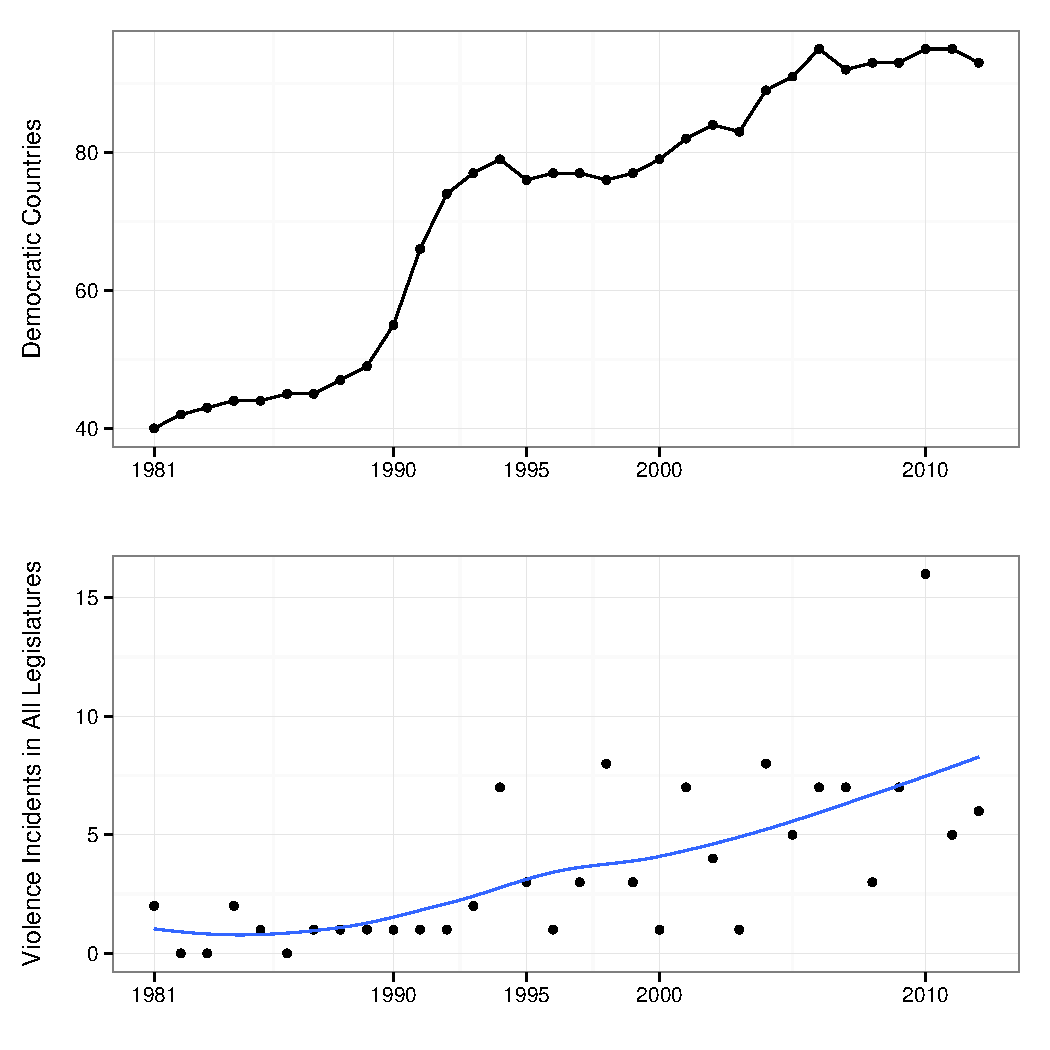
\includegraphics[width=0.8\linewidth]{figure/compareLegToViolence-1} 

\end{knitrout}
    \end{center}

    \caption{Comparing the Number of Democracies to Observed Violence in All Legislatures Over Time (1981-2012)}
    \label{elect_vs_violence}

\end{figure}

\section*{Discussion of Contrasting Contemporary Cases}

\todo[inline]{This paragraph was moved from the main text to meet word limit requirements.}

While it appears in Figure 2 of the article's main text that having disproportionate electoral outcomes \emph{or} a new democracy is not necessary for legislative violence, based on the data, having \emph{both} of them might make violence much more likely. South Korea's national assembly, like the antebellum US Senate, is an example of a `perfect storm'. It is both in a new democracy and has relatively disproportionate electoral outcomes.\footnote{South Korea's average disproportionality as measured by the Gallagher Index \citep{Gallagher1991} from 2000 until 2012 was 12. This places it in the upper 25\% of observations with elected legislatures. It also became a democracy within the past 20 years.} South Korea had eight observed incidents of legislative violence in the full sample. Countries that have \emph{either} proportional outcomes \emph{or} old democracies appear to be able to compensate fairly well for an absence of the other characteristic. The United Kingdom has a relatively disproportionate electoral system,\footnote{It had an average Gallagher disproportionality of 16.5 from 2000 to 2012.} but no violence in the sample. One reason for this might be that it has a very old democracy where the major parties have had experience in government and so view commitments to allow for the alteration of power to be credible. Conversely, only one incident of violence\footnote{Two members of parliament punched each other in 1998.} was observed in South Africa's new democracy during the sampling period. South Africa's democracy is about the same age as South Korea's and the country has a very violent recent past and present,\footnote{Its rate of murders per 100,000 people is regularly among the highest in the \cite{UNMurder2013} data set.} but it has very proportionate electoral outcomes.\footnote{South Africa's average disproportionality was 0.28 from 2000 until 2012, one of the lowest observed in the sample.} South Africa's one scuffle in 1998 is quite an outlier as it is the only violent incident observed in very proportional legislatures in the sample.\footnote{There was a scuffle in the South African legislature on 12 February 2015, when opposition legislators were being ejected for interrupting the president \citep{Guardian2015}. Though South Africa has very proportionate electoral outcomes, the ruling African National Congress' uninterrupted rule since the end of Apartheid is perhaps beginning to test opposition legislators' belief that the majority can maintain its commitments, especially to alternate power.}

\section*{Additional Right-hand Variables}

\todo[inline]{This section was moved from the main text at the editor's request}

I examined a number of other legislative and societal-level variables to guard against omitted variable bias. Results from models with these variables are shown in tables \ref{outputTable.dem} and \ref{outputTable.1990_2nd}. The variables are described below. It is important to first note that overall these factors were not found to be statistically significantly associated with legislative violence nor did they substantively alter the article's core findings.

I avoid focusing on models that include highly correlated variables \citep[]{Achen2002, Schrodt2006}. In these models (not shown), as the statistical literature predicts, the coefficient estimates and standard errors change dramatically for many of the variables. Earlier models included a government system type variable. However, I ignore results from this variable. It had very large, highly unstable, and largely nonsensical coefficient estimates, suggesting that the model does not contain enough information to test \citep{Babyak2004} whether or not crude political system type has an effect on violence. \add{The instability in the coefficient estimates likely has more to do with a lack of variation on this covariate rather than the violence dependent variable. Political systems rarely change in the sample of democracies.}

\subsubsection*{Motivation and Variable Descriptions}

\todo[inline]{The following paragraph was added. Subsequent paragraphs are from the original.}

Previous research on protest movements has often focused on how they organize to overcome the collective action problems that would discourage individuals from protesting \citep{lohmann1994,tucker2007}. Perhaps this approach is applicable to legislative violence. Groups of legislators that are better able to organize may be more willing and able to engage in violent acts. However, there is a clear reason to be sceptical of the usefulness of this approach to explain whether or not legislative brawls occur: legislators are generally well-organized into political parties. Even weak parties with few members (typically in the hundreds at most) relative to protest movements are generally better organized and less subject to collective action problems than protest movements. That being said, the legislative studies literature has shown that the degree of personal vs. party organization varies considerably across countries and is particularly influenced by the electoral system \citep{carey1995}. For example, if parties control the order of candidates on a closed-list ballot then the party will have considerable control over politicians. If a politician does not tow the party line, then the party could move the candidate lower down the list at the next election, decreasing their chances of re-election. Conversely, if candidates are placed on the ballot through open primaries, then parties have fewer sticks to control legislators, who instead have stronger incentives to cultivate a personal vote. Legislative collective action problems in these systems are higher. To measure the degree of party control I used data on \emph{personal vote} rank in countries's dominant legislative tier--i.e. the chamber with the most seats. The data is from \cite{johnson2012} and is based on the index developed by \cite{carey1995}. Scores range between 1 and 13. Higher scores indicate stronger incentives for candidates to cultivate a personal vote, i.e. there is less party control. The data is available through 2005. I assumed it was constant from this point through 2012.

Gender is closely correlated with violence in society generally. Though there are many possible reasons for this that are beyond the scope of this article, women tend to commit many fewer acts of violence than men \citep[]{Schwartz2009}. Previous research has found that women's participation in parliament has an impact on government decisions to go to war \citep{Melander2005}. Perhaps if a larger proportion of legislators are women there will be less violence in the parliamentary chamber. To examine this possibility, I gathered data on the \emph{percentage of women in parliament} per country-year from two sources. Data from 1997 and after was from the Inter-Parliamentary Union \citeyearpar{IPU2013} via the \cite{WorldBank2011}. Data from before 1997 was from \cite{Schwartz2009}.

I included countries' \emph{murder rate}, i.e. murders per 100,000 people, to measure a possible association between societal-level and legislative violence. The data was from \cite{UNMurder2013}, which aggregated annual murder rates from a variety of national and international sources. The data is available from 1995 through 2011.\footnote{Beyond truncating the sample somewhat, this data set unfortunately does not record Taiwan's murder rate separately from China's.}

I also included standard measures of the \emph{effective number of parliamentary parties} by votes and by seats \citep[]{Laakso1979, Taagepera1989}. The data was taken from \cite{Carey2011} before 2004 and from \cite{Gallagher2012} afterwards. Both of these measures indicate how fragmented a parliamentary party system is. Higher scores indicate that there are more parties that win either votes or seats. Neither measure produced statistically significant results, so only the results for the effective number of parties by seats are shown below.

To examine whether or not national legislative losers may be dissuaded from legislative violence because there is a possibility of gaining power at a provincial-level, I include the \emph{federalism} dummy variable from \cite{Carey2011}. I updated this from 2004 until the end of the observation period. In early models I also controlled for the government system type, i.e. if it had a presidential, parliamentary, or mixed assembly-elected presidential. This was from the Database of Political Institutions (DPI) \citep[updated through 2012]{DPI2001}.

Conflict in more economically divided societies may be generally more intense. These conflicts may spill over into legislatures where they precipitate violence between members. To capture effects of economic divisions, I include {\emph{Gini coefficients of economic inequality}} from \cite{UNU2008}.\footnote{Note, for country-years with missing data I assumed that the Gini Coefficient remained constant from the last year there is data for the country, unless the span was ten years or more. If this was the case they were treated as missing.} Finally, as is common in cross-country analyses, I also include the natural logarithm (due to its right-skewed distribution) of {\emph{gross domestic product per capita}}. This data is from the World Bank's International Development Indicators \citeyearpar{WorldBank2011} and is in thousands of 2005 United States dollars.

\subsection*{Results Discussion}

\todo[inline]{Moved from main paper and changed for results with updated data.}

\paragraph{Societal-level Variables}

In general the additional societal-level variables were found to be associated with legislative violence in any of the models. Countries' murder rates were not found to be associated with violence indicating that the link between societal and legislative violence is not strong. GDP per capita was also not found to be associated with violence. The Gini coefficient was negatively associated with brawls--more inequality was associated with less violence. This finding runs counter to expectations and requires more research to fully understand. Nonetheless, the article's core findings remain the same when Gini is included.

\paragraph{Other Political and Institutional Variables}

Results for other political and institutional variables were largely not statistically significant. The personalistic vote index was insignificant, perhaps because the baseline level of party organization is high, even if it does vary between legislatures. The effective number of parties variables and the basic continuous government fractionalization variable was statistically significant in the analyses. Likewise, federalism did not appear to be robustly related to legislative violence across the models. All of these variables are not as directly related to an ability to make credible legislative commitments at a theoretical level, compared to disproportionality, democratic age and, to a lesser extent, governing majority size. So it should not come as too much of a surprise to find that they are not associated with legislative violence in these models.


%%%%%%%% Elected Legislatures Results Table
\begin{table}[H]
\caption{Legislative Violence Rare Events Logistic Regression Results (Multi-Party Elected Legislature 1981-2012)}
\label{outputTable.dem}
\begin{center}
{\scalebox{0.45}{

% Table created by stargazer v.5.1 by Marek Hlavac, Harvard University. E-mail: hlavac at fas.harvard.edu
% Date and time: Tue, Apr 14, 2015 - 07:42:11
\begin{tabular}{@{\extracolsep{5pt}}lcccccccccccc} 
\\[-1.8ex]\hline 
\hline \\[-1.8ex] 
 & \multicolumn{12}{c}{\textit{Dependent variable:}} \\ 
\cline{2-13} 
\\[-1.8ex] & \multicolumn{12}{c}{Violent Incident} \\ 
\\[-1.8ex] & (1) & (2) & (3) & (4) & (5) & (6) & (7) & (8) & (9) & (10) & (11) & (12)\\ 
\hline \\[-1.8ex] 
 Lower Disproportionality & $-$0.701$^{***}$ & $-$0.689$^{***}$ & $-$0.693$^{***}$ & $-$0.664$^{**}$ & $-$0.524$^{*}$ & $-$0.722$^{**}$ & $-$0.732$^{**}$ & $-$0.883$^{**}$ & $-$0.692$^{**}$ & $-$0.587$^{**}$ & $-$0.652$^{**}$ & $-$0.524$^{*}$ \\ 
  & (0.266) & (0.266) & (0.267) & (0.266) & (0.297) & (0.302) & (0.306) & (0.393) & (0.274) & (0.272) & (0.266) & (0.279) \\ 
  & & & & & & & & & & & & \\ 
 Dem. Age (log) & $-$0.303$^{***}$ & $-$0.297$^{***}$ & $-$0.299$^{***}$ & $-$0.294$^{***}$ & $-$0.340$^{***}$ & $-$0.374$^{***}$ & $-$0.336$^{***}$ & $-$0.344$^{**}$ & $-$0.325$^{***}$ & $-$0.332$^{***}$ & $-$0.350$^{***}$ & $-$0.301$^{**}$ \\ 
  & (0.105) & (0.105) & (0.107) & (0.105) & (0.127) & (0.116) & (0.121) & (0.162) & (0.117) & (0.112) & (0.105) & (0.128) \\ 
  & & & & & & & & & & & & \\ 
 Majority Size & $-$0.023$^{***}$ & $-$0.023$^{***}$ & $-$0.023$^{***}$ & $-$0.022$^{***}$ & $-$0.019$^{*}$ & $-$0.029$^{***}$ & $-$0.022$^{**}$ & $-$0.028$^{**}$ & $-$0.026$^{***}$ & $-$0.026$^{***}$ & $-$0.024$^{***}$ & $-$0.020$^{**}$ \\ 
  & (0.008) & (0.008) & (0.008) & (0.008) & (0.010) & (0.009) & (0.009) & (0.014) & (0.009) & (0.009) & (0.009) & (0.009) \\ 
  & & & & & & & & & & & & \\ 
 Internal Armed Conflict &  & 0.556$^{*}$ & 0.535$^{*}$ & 0.542$^{*}$ & 0.494 & 0.629$^{*}$ & 0.689$^{**}$ & 0.189 & 0.537$^{*}$ & 0.576$^{*}$ & 0.638$^{**}$ & 0.661$^{**}$ \\ 
  &  & (0.303) & (0.303) & (0.303) & (0.350) & (0.371) & (0.336) & (0.547) & (0.309) & (0.308) & (0.308) & (0.316) \\ 
  & & & & & & & & & & & & \\ 
 Leg. Immunity &  &  & $-$0.015 &  &  &  &  &  &  &  &  &  \\ 
  &  &  & (0.257) &  &  &  &  &  &  &  &  &  \\ 
  & & & & & & & & & & & & \\ 
 Single Party Gov. &  &  & $-$0.102 &  &  &  &  &  &  &  &  &  \\ 
  &  &  & (0.249) &  &  &  &  &  &  &  &  &  \\ 
  & & & & & & & & & & & & \\ 
 Political Constraints &  &  &  & $-$0.735 &  &  &  &  &  &  &  &  \\ 
  &  &  &  & (0.912) &  &  &  &  &  &  &  &  \\ 
  & & & & & & & & & & & & \\ 
 Self Expression &  &  &  &  & 2.384 &  &  &  &  &  &  &  \\ 
  &  &  &  &  & (2.432) &  &  &  &  &  &  &  \\ 
  & & & & & & & & & & & & \\ 
 Ethnic Frac. &  &  &  &  & $-$0.523 &  &  &  &  &  &  &  \\ 
  &  &  &  &  & (0.762) &  &  &  &  &  &  &  \\ 
  & & & & & & & & & & & & \\ 
 Personalistic Vote &  &  &  &  &  & 0.018 &  &  &  &  &  &  \\ 
  &  &  &  &  &  & (0.038) &  &  &  &  &  &  \\ 
  & & & & & & & & & & & & \\ 
 Perc. Women in Parl. &  &  &  &  &  &  & 0.015 &  &  &  &  &  \\ 
  &  &  &  &  &  &  & (0.017) &  &  &  &  &  \\ 
  & & & & & & & & & & & & \\ 
 Murder Rate &  &  &  &  &  &  &  & $-$0.002 &  &  &  &  \\ 
  &  &  &  &  &  &  &  & (0.013) &  &  &  &  \\ 
  & & & & & & & & & & & & \\ 
 Federal &  &  &  &  &  &  &  &  & 0.132 &  &  &  \\ 
  &  &  &  &  &  &  &  &  & (0.357) &  &  &  \\ 
  & & & & & & & & & & & & \\ 
 Gov. Frac. &  &  &  &  &  &  &  &  & 0.083 &  &  &  \\ 
  &  &  &  &  &  &  &  &  & (0.468) &  &  &  \\ 
  & & & & & & & & & & & & \\ 
 No. of Parties by Seats &  &  &  &  &  &  &  &  &  & $-$0.091 &  &  \\ 
  &  &  &  &  &  &  &  &  &  & (0.093) &  &  \\ 
  & & & & & & & & & & & & \\ 
 GINI &  &  &  &  &  &  &  &  &  &  & $-$0.040$^{***}$ &  \\ 
  &  &  &  &  &  &  &  &  &  &  & (0.015) &  \\ 
  & & & & & & & & & & & & \\ 
 GDP per Capita (log) &  &  &  &  &  &  &  &  &  &  &  & $-$0.048 \\ 
  &  &  &  &  &  &  &  &  &  &  &  & (0.120) \\ 
  & & & & & & & & & & & & \\ 
 (Intercept) & $-$0.831 & $-$0.923$^{*}$ & $-$0.835 & $-$0.717 & $-$3.897 & $-$0.417 & $-$1.067$^{*}$ & $-$0.288 & $-$0.688 & $-$0.371 & 0.775 & $-$1.085$^{*}$ \\ 
  & (0.534) & (0.538) & (0.633) & (0.604) & (3.040) & (0.565) & (0.623) & (0.807) & (0.572) & (0.730) & (0.826) & (0.580) \\ 
  & & & & & & & & & & & & \\ 
\hline \\[-1.8ex] 
Observations & 1,707 & 1,707 & 1,682 & 1,682 & 911 & 1,495 & 1,586 & 821 & 1,570 & 1,591 & 1,684 & 1,628 \\ 
Log Likelihood & $-$279.636 & $-$278.226 & $-$277.253 & $-$277.151 & $-$203.983 & $-$238.522 & $-$226.651 & $-$134.936 & $-$259.188 & $-$263.690 & $-$273.029 & $-$248.318 \\ 
Akaike Inf. Crit. & 567.272 & 566.452 & 568.507 & 566.302 & 421.966 & 489.043 & 465.303 & 281.872 & 532.377 & 539.380 & 558.058 & 508.636 \\ 
\hline 
\hline \\[-1.8ex] 
\multicolumn{13}{l}{$^{*}$p$<$0.1; $^{**}$p$<$0.05; $^{***}$p$<$0.01} \\ 
\multicolumn{13}{l}{Standard errors are in parentheses. All models use robust (WEAVE) standard errors.} \\ 
\end{tabular} 

}}
\end{center}

\end{table}

%%%%%%%% Elected Legislatures Results Table from 1990--Robustness
\begin{table}[H]
\caption{Legislative Violence Regression Results (Democratic Legislature from 1990-2012)}
\label{outputTable.1990_2nd}
\begin{center}
\scalebox{0.5}{

% Table created by stargazer v.5.1 by Marek Hlavac, Harvard University. E-mail: hlavac at fas.harvard.edu
% Date and time: Tue, Apr 14, 2015 - 07:42:16
\begin{tabular}{@{\extracolsep{5pt}}lccccccc} 
\\[-1.8ex]\hline 
\hline \\[-1.8ex] 
 & \multicolumn{7}{c}{\textit{Dependent variable:}} \\ 
\cline{2-8} 
\\[-1.8ex] & \multicolumn{7}{c}{Violent Incident} \\ 
\\[-1.8ex] & (1) & (2) & (3) & (4) & (5) & (6) & (7)\\ 
\hline \\[-1.8ex] 
 Lower Disproportionality & $-$0.592$^{*}$ & $-$0.588$^{*}$ & $-$0.883$^{**}$ & $-$0.602$^{**}$ & $-$0.506$^{*}$ & $-$0.543$^{**}$ & $-$0.429 \\ 
  & (0.308) & (0.313) & (0.393) & (0.278) & (0.276) & (0.271) & (0.286) \\ 
  & & & & & & & \\ 
 Dem. Age (log) & $-$0.375$^{***}$ & $-$0.368$^{***}$ & $-$0.344$^{**}$ & $-$0.356$^{***}$ & $-$0.372$^{***}$ & $-$0.367$^{***}$ & $-$0.450$^{***}$ \\ 
  & (0.122) & (0.130) & (0.162) & (0.126) & (0.119) & (0.110) & (0.139) \\ 
  & & & & & & & \\ 
 Majority Size & $-$0.030$^{***}$ & $-$0.021$^{**}$ & $-$0.028$^{**}$ & $-$0.024$^{**}$ & $-$0.025$^{***}$ & $-$0.023$^{**}$ & $-$0.019$^{**}$ \\ 
  & (0.010) & (0.010) & (0.014) & (0.009) & (0.010) & (0.009) & (0.009) \\ 
  & & & & & & & \\ 
 Internal Armed Conflict & 0.324 & 0.509 & 0.188 & 0.452 & 0.504 & 0.549 & 0.648$^{*}$ \\ 
  & (0.432) & (0.386) & (0.547) & (0.352) & (0.351) & (0.351) & (0.358) \\ 
  & & & & & & & \\ 
 Personalistic Vote & 0.016 &  &  &  &  &  &  \\ 
  & (0.039) &  &  &  &  &  &  \\ 
  & & & & & & & \\ 
 Perc. Women in Parliament &  & 0.009 &  &  &  &  &  \\ 
  &  & (0.019) &  &  &  &  &  \\ 
  & & & & & & & \\ 
 Murder Rate &  &  & $-$0.002 &  &  &  &  \\ 
  &  &  & (0.013) &  &  &  &  \\ 
  & & & & & & & \\ 
 Federal &  &  &  & $-$0.036 &  &  &  \\ 
  &  &  &  & (0.410) &  &  &  \\ 
  & & & & & & & \\ 
 Gov. Frac. &  &  &  & $-$0.066 &  &  &  \\ 
  &  &  &  & (0.489) &  &  &  \\ 
  & & & & & & & \\ 
 No. of Parties by Seats &  &  &  &  & $-$0.123 &  &  \\ 
  &  &  &  &  & (0.098) &  &  \\ 
  & & & & & & & \\ 
 Gini &  &  &  &  &  & $-$0.043$^{***}$ &  \\ 
  &  &  &  &  &  & (0.016) &  \\ 
  & & & & & & & \\ 
 GDP per Capita (log) &  &  &  &  &  &  & 0.137 \\ 
  &  &  &  &  &  &  & (0.132) \\ 
  & & & & & & & \\ 
 (Intercept) & $-$0.272 & $-$0.861 & $-$0.177 & $-$0.564 & $-$0.112 & 0.971 & $-$0.939 \\ 
  & (0.598) & (0.652) & (0.807) & (0.597) & (0.764) & (0.849) & (0.612) \\ 
  & & & & & & & \\ 
\hline \\[-1.8ex] 
Observations & 1,291 & 1,320 & 821 & 1,319 & 1,337 & 1,418 & 1,371 \\ 
Log Likelihood & $-$220.241 & $-$203.253 & $-$134.936 & $-$235.109 & $-$238.861 & $-$247.922 & $-$223.698 \\ 
Akaike Inf. Crit. & 452.482 & 418.507 & 281.872 & 484.219 & 489.722 & 507.845 & 459.396 \\ 
\hline 
\hline \\[-1.8ex] 
\multicolumn{8}{l}{$^{*}$p$<$0.1; $^{**}$p$<$0.05; $^{***}$p$<$0.01} \\ 
\multicolumn{8}{l}{Standard errors are in parentheses. All models use robust (WEAVE) standard errors.} \\ 
\end{tabular} 

}
\end{center}
\end{table}

\section*{Details on Prior Correction of the Rare Logistic Regression Models}

For prior correction \citep[see][]{KingRareEventsPA2001} in the models with the full sample of democratic legislatures I used the observed proportion of all observations with legislative violence \change{up to 2010}{through 2012}: i.e. \change{2.1}{3.7} percent of observations up until \change{2010}{2012} had violence ($\tau = \frac{86}{2297} = 0.037$). There were \change{63}{79} observed incidents of violence and \change{2654}{1898} country-years from 1990 through \change{2009}{2012} in the sample, so: $\tau = \frac{79}{1898} = 0.042$.

\section*{Interactions}

\todo[inline]{Section added}

While I did not find evidence for additive relationships between most of the societal variables and legislative brawls, perhaps they mediate the effect of disproportionality or democratic age. For example, legislators in more homogeneous societies might have fewer information asymmetries across partisan divides, thus enabling them to establish credible commitments in new democracies. Tables \ref{prop_interact} and \ref{dem_interact} provide the raw estimates from these interactive models. We can see that some of the interactions contain statistically significant terms, though often only at the 10\% level.

As in the main article, in order to evaluate the substantive significance of these findings I simulated expected probabilities for interactions that included statistically significant terms at the 5\% level and higher. I then plotted them in figures \ref{interact_plots1} and \ref{interact_plots2}.\footnote{See Figure \ref{marginal_effect_plot} for marginal effects \citep{Brambor2006}. The substantive importance of the interactions is not conveyed as effectively in these plots. In addition, while the interaction between lower disproportionality and the Gini coefficient contains significant terms at the 5\% level the effect is substantively meaningless and is not plotted.} The plots show expected probabilities for various levels of low disproportionality and democratic age at `high' and `low' values of the other variables in the interactions. Self-expression was high at 1.35 and low at 1.1. Ethnic fractionalization was high at 0.8 and low at 0.1. Finally, political constraints were high at 0.7 and low at 0.1. These fitted values are close to the variables' minimum and maximum values to enable the largest meaningful contrasts.

The substantive importance of these interactions is overall very weak. Plots of the simulations illustrate that there is considerable overlap in the uncertainty surrounding most of the estimates for substantively meaningful fitted values. This is especially true for interactions with the low disproportionality variable. To the extent that the estimates are suggestive of true interactive effects, overall it appears that factors creating credible commitment problems in new democracies are worsened by ethnic divisions and few constraints on altering policy. The top-panel of Figure \ref{dem_interact} suggests that perhaps in new democracies violence is more likely when there is more ethnic fictionalization. Credible commitment problems between ethnic groups could be particularly strong in these countries. The bottom-panel of Figure \ref{dem_interact} suggests that high political constraints on policy change mediate the effect of democratic age on violence. Having more and more disperse veto players make it difficult for the current majority to enact policy change, perhaps improving their ability to make credible commitments.

It is important to reiterate that though these interactive effects have statistically significant terms, the substantive importance of these estimates for meaningful fitted values is very weak.

\begin{figure}[H]
    \begin{center}
\begin{knitrout}
\definecolor{shadecolor}{rgb}{0.969, 0.969, 0.969}\color{fgcolor}
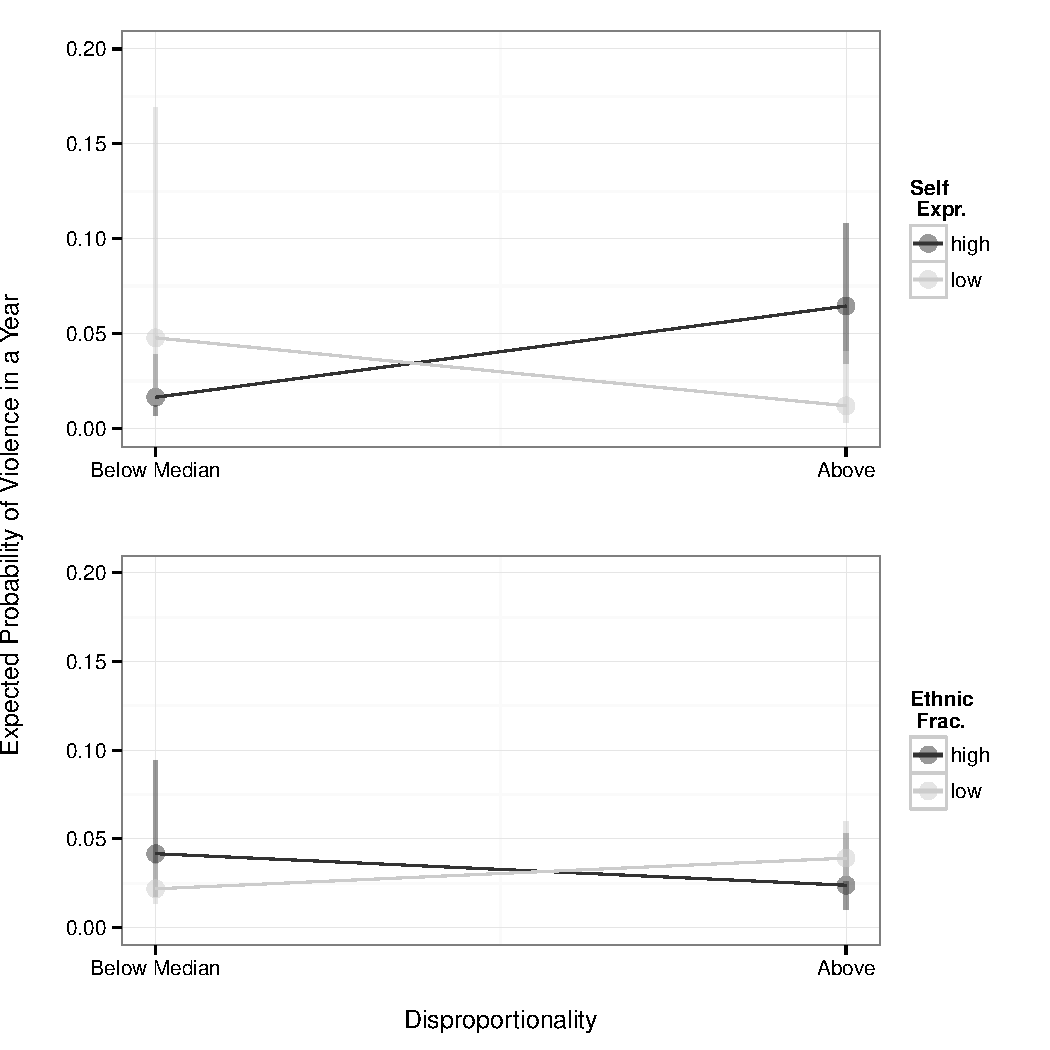
\includegraphics[width=0.95\linewidth]{figure/predProInteract1-1} 

\end{knitrout}

    \end{center}
    \caption{Expected Probability of Legislative Violence in Democratic Legislatures per Year (Interactions 1)}
    \label{interact_plots1}
    \begin{singlespace}
      {\scriptsize{The graphs show the median and middle 95\% of 1000 simulations at each fitted value of the variables. The simulations use estimates from tables \ref{prop_interact} and \ref{dem_interact}. For each set of simulations all other variables were fitted at their means.}}
    \end{singlespace}
\end{figure}

\begin{figure}[H]
    \begin{center}
\begin{knitrout}
\definecolor{shadecolor}{rgb}{0.969, 0.969, 0.969}\color{fgcolor}
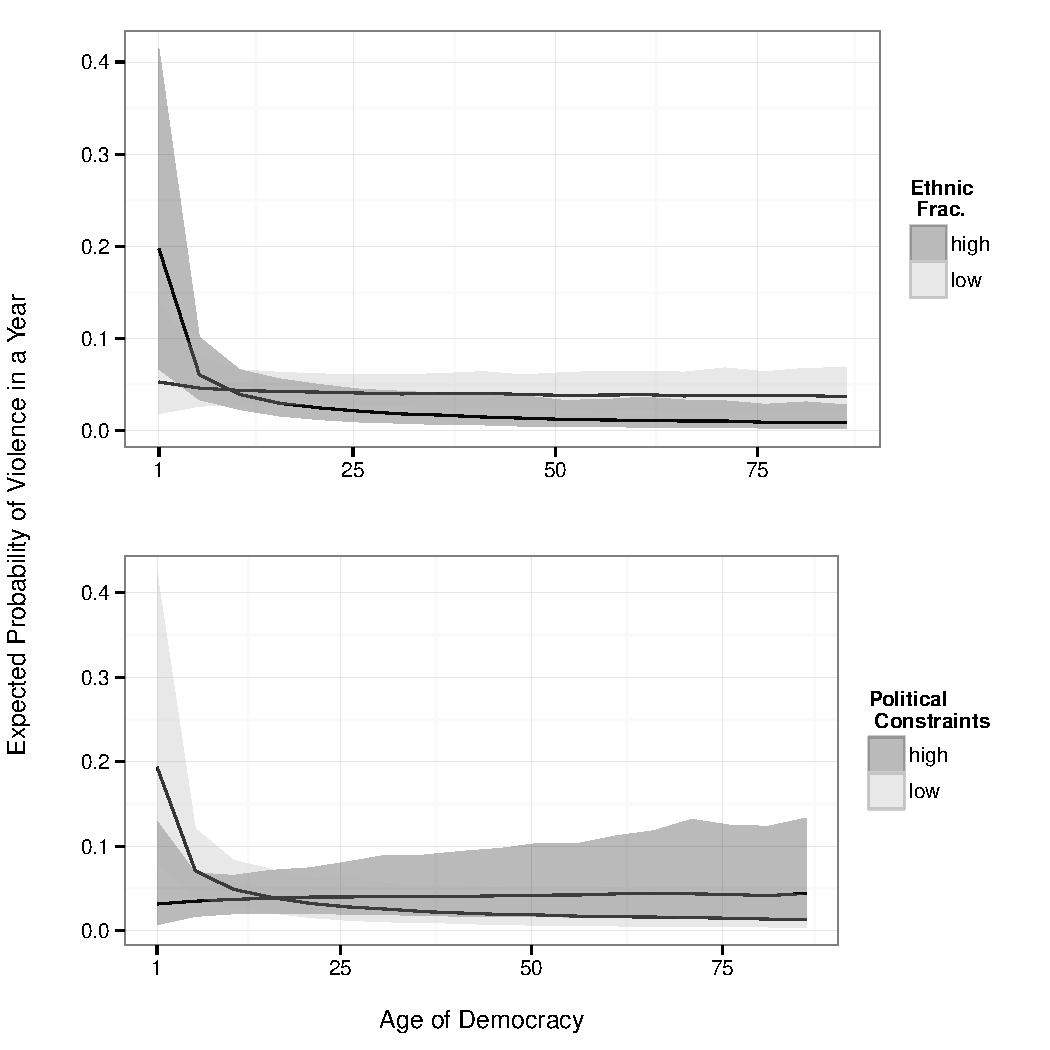
\includegraphics[width=0.95\linewidth]{figure/predProInteract2-1} 

\end{knitrout}

    \end{center}
    \caption{Expected Probability of Legislative Violence in Democratic Legislatures per Year (Interactions 2)}
    \label{interact_plots2}
    \begin{singlespace}
      {\scriptsize{The graphs show the median and middle 95\% of 1000 simulations at each fitted value of the variables. The simulations use estimates from tables \ref{prop_interact} and \ref{dem_interact}. For each set of simulations all other variables were fitted at their means.}}
    \end{singlespace}
\end{figure}

\begin{table}[H]
    \caption{Legislative Violence Regression Results with Lower Disproportionality Interactions (Democratic Legislature from 1990-2012)}
    \label{prop_interact}
    \begin{center}
    \scalebox{0.7}{

% Table created by stargazer v.5.1 by Marek Hlavac, Harvard University. E-mail: hlavac at fas.harvard.edu
% Date and time: Tue, Apr 14, 2015 - 07:42:22
\begin{tabular}{@{\extracolsep{5pt}}lcccccc} 
\\[-1.8ex]\hline 
\hline \\[-1.8ex] 
 & \multicolumn{6}{c}{\textit{Dependent variable:}} \\ 
\cline{2-7} 
\\[-1.8ex] & \multicolumn{6}{c}{Violent Incident} \\ 
\\[-1.8ex] & (1) & (2) & (3) & (4) & (5) & (6)\\ 
\hline \\[-1.8ex] 
 Majority Size & $-$0.022$^{**}$ & $-$0.017$^{*}$ & $-$0.022$^{**}$ & $-$0.023$^{**}$ & $-$0.018$^{*}$ & $-$0.020$^{**}$ \\ 
  & (0.009) & (0.010) & (0.009) & (0.009) & (0.010) & (0.009) \\ 
  & & & & & & \\ 
 Dem. Age (log) & $-$0.245$^{*}$ & $-$0.384$^{***}$ & $-$0.335$^{***}$ & $-$0.373$^{***}$ & $-$0.412$^{***}$ & $-$0.329$^{***}$ \\ 
  & (0.137) & (0.132) & (0.114) & (0.112) & (0.142) & (0.112) \\ 
  & & & & & & \\ 
 Lower Disproportionality & 0.082 & 14.407$^{**}$ & $-$1.638$^{***}$ & $-$0.559 & 0.262 & 0.022 \\ 
  & (0.654) & (6.481) & (0.588) & (1.168) & (0.431) & (0.765) \\ 
  & & & & & & \\ 
 Lower Disp.*Dem. Age & $-$0.252 &  &  &  &  &  \\ 
  & (0.234) &  &  &  &  &  \\ 
  & & & & & & \\ 
 Self Expression &  & 7.058$^{**}$ &  &  &  &  \\ 
  &  & (3.210) &  &  &  &  \\ 
  & & & & & & \\ 
 Lower Disp.*Self Expression &  & $-$11.738$^{**}$ &  &  &  &  \\ 
  &  & (5.128) &  &  &  &  \\ 
  & & & & & & \\ 
 Ethnic Frac. &  &  & $-$1.193 &  &  &  \\ 
  &  &  & (0.758) &  &  &  \\ 
  & & & & & & \\ 
 Lower Disp.*Ethnic Frac. &  &  & 2.776$^{**}$ &  &  &  \\ 
  &  &  & (1.270) &  &  &  \\ 
  & & & & & & \\ 
 GINI &  &  &  & $-$0.039$^{*}$ &  &  \\ 
  &  &  &  & (0.021) &  &  \\ 
  & & & & & & \\ 
 Lower Disp.*GINI &  &  &  & 0.001 &  &  \\ 
  &  &  &  & (0.030) &  &  \\ 
  & & & & & & \\ 
 GDP per Capita (log) &  &  &  &  & 0.244 &  \\ 
  &  &  &  &  & (0.153) &  \\ 
  & & & & & & \\ 
 Lower Disp.*GDP Per Capita &  &  &  &  & $-$0.449$^{*}$ &  \\ 
  &  &  &  &  & (0.231) &  \\ 
  & & & & & & \\ 
 Political Constraints &  &  &  &  &  & $-$0.030 \\ 
  &  &  &  &  &  & (1.169) \\ 
  & & & & & & \\ 
 Lower Disp.*Pol. Constraints &  &  &  &  &  & $-$1.483 \\ 
  &  &  &  &  &  & (1.881) \\ 
  & & & & & & \\ 
 (Intercept) & $-$0.953 & $-$9.836$^{**}$ & $-$0.313 & 0.928 & $-$1.177$^{*}$ & $-$0.850 \\ 
  & (0.597) & (4.097) & (0.653) & (0.982) & (0.648) & (0.728) \\ 
  & & & & & & \\ 
\hline \\[-1.8ex] 
Observations & 1,441 & 810 & 1,435 & 1,418 & 1,371 & 1,417 \\ 
Log Likelihood & $-$253.644 & $-$186.409 & $-$251.423 & $-$248.923 & $-$222.992 & $-$252.849 \\ 
Akaike Inf. Crit. & 517.288 & 384.817 & 514.846 & 509.845 & 457.984 & 517.697 \\ 
\hline 
\hline \\[-1.8ex] 
\multicolumn{7}{l}{$^{*}$p$<$0.1; $^{**}$p$<$0.05; $^{***}$p$<$0.01} \\ 
\multicolumn{7}{l}{Standard errors are in parentheses. All models use robust (WEAVE) standard errors.} \\ 
\end{tabular} 

    }
    \end{center}
\end{table}

}
\begin{table}[H]
    \caption{Legislative Violence Regression Results with Democratic Age Interactions (Democratic Legislature from 1990-2012)}
    \label{dem_interact}
    \begin{center}
    \scalebox{0.7}{

% Table created by stargazer v.5.1 by Marek Hlavac, Harvard University. E-mail: hlavac at fas.harvard.edu
% Date and time: Tue, Apr 14, 2015 - 07:42:24
\begin{tabular}{@{\extracolsep{5pt}}lccccc} 
\\[-1.8ex]\hline 
\hline \\[-1.8ex] 
 & \multicolumn{5}{c}{\textit{Dependent variable:}} \\ 
\cline{2-6} 
\\[-1.8ex] & \multicolumn{5}{c}{Violent Incident} \\ 
\\[-1.8ex] & (1) & (2) & (3) & (4) & (5)\\ 
\hline \\[-1.8ex] 
 Majority Size & $-$0.019$^{*}$ & $-$0.023$^{***}$ & $-$0.023$^{**}$ & $-$0.019$^{**}$ & $-$0.024$^{***}$ \\ 
  & (0.010) & (0.009) & (0.009) & (0.009) & (0.009) \\ 
  & & & & & \\ 
 Lower Disproportionality & $-$0.465 & $-$0.583$^{**}$ & $-$0.537$^{**}$ & $-$0.410 & $-$0.568$^{**}$ \\ 
  & (0.301) & (0.271) & (0.272) & (0.285) & (0.272) \\ 
  & & & & & \\ 
 Dem. Age (log) & $-$0.749 & 0.018 & 0.008 & $-$0.364$^{*}$ & $-$0.780$^{**}$ \\ 
  & (2.750) & (0.213) & (0.503) & (0.207) & (0.313) \\ 
  & & & & & \\ 
 Self Expression & 2.873 &  &  &  &  \\ 
  & (5.389) &  &  &  &  \\ 
  & & & & & \\ 
 Dem. Age*Self Expression & 0.277 &  &  &  &  \\ 
  & (2.139) &  &  &  &  \\ 
  & & & & & \\ 
 Ethnic Frac. &  & 2.155 &  &  &  \\ 
  &  & (1.340) &  &  &  \\ 
  & & & & & \\ 
 Dem. Age*Ethnic Frac. &  & $-$0.971$^{**}$ &  &  &  \\ 
  &  & (0.486) &  &  &  \\ 
  & & & & & \\ 
 GINI &  &  & $-$0.015 &  &  \\ 
  &  &  & (0.034) &  &  \\ 
  & & & & & \\ 
 Dem. Age*GINI &  &  & $-$0.010 &  &  \\ 
  &  &  & (0.013) &  &  \\ 
  & & & & & \\ 
 GDP per Capita (log) &  &  &  & 0.209 &  \\ 
  &  &  &  & (0.283) &  \\ 
  & & & & & \\ 
 Dem. Age*GDP Per Capita &  &  &  & $-$0.042 &  \\ 
  &  &  &  & (0.092) &  \\ 
  & & & & & \\ 
 Political Constraints &  &  &  &  & $-$3.405$^{*}$ \\ 
  &  &  &  &  & (1.983) \\ 
  & & & & & \\ 
 Dem. Age*Pol. Constraints &  &  &  &  & 1.224 \\ 
  &  &  &  &  & (0.786) \\ 
  & & & & & \\ 
 (Intercept) & $-$4.392 & $-$1.535$^{*}$ & 0.046 & $-$0.997 & 0.574 \\ 
  & (6.876) & (0.806) & (1.396) & (0.739) & (0.960) \\ 
  & & & & & \\ 
\hline \\[-1.8ex] 
Observations & 810 & 1,435 & 1,418 & 1,371 & 1,417 \\ 
Log Likelihood & $-$189.097 & $-$252.058 & $-$248.643 & $-$224.856 & $-$252.091 \\ 
Akaike Inf. Crit. & 390.194 & 516.115 & 509.285 & 461.711 & 516.183 \\ 
\hline 
\hline \\[-1.8ex] 
\multicolumn{6}{l}{$^{*}$p$<$0.1; $^{**}$p$<$0.05; $^{***}$p$<$0.01} \\ 
\multicolumn{6}{l}{Standard errors are in parentheses. All models use robust (WEAVE) standard errors.} \\ 
\end{tabular} 

    }
    \end{center}
\end{table}

\begin{figure}[H]
    \begin{center}
\begin{knitrout}
\definecolor{shadecolor}{rgb}{0.969, 0.969, 0.969}\color{fgcolor}
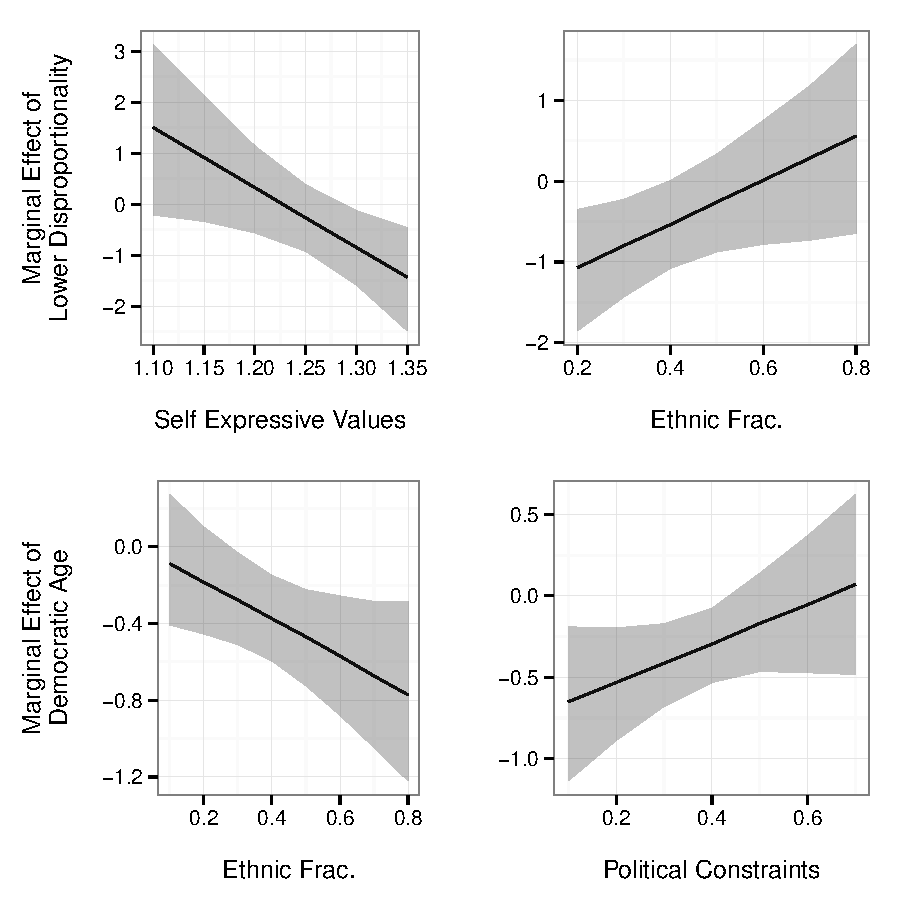
\includegraphics[width=0.95\linewidth]{figure/marginalEffects-1} 

\end{knitrout}
    \end{center}
    \caption{Marginal Effects of Lower Disproportionality and Democratic Age Given Representative Ranges of Interaction Variables}
    \label{marginal_effect_plot}
    \begin{singlespace}
      {\scriptsize{The graphs show the median and middle 95\% of 1000 simulations at each fitted value of the variables. The simulations use estimates from tables \ref{prop_interact} and \ref{dem_interact}.}}
    \end{singlespace}
\end{figure}


\section*{Ethnic fractionalization list-wise inclusion}

\todo[inline]{Section added.}

Table \ref{results_frac} shows models with ethnic fractionalization where key variables from the analysis are list-wise included. Ethnic fractionalization is statistically significantly associated with violence at the 10\% level in two of these models. However, there are a number of reasons to be very sceptical of this result. First, the direction of the estimated effect runs strongly counter to our expectations in that more fractionalization is associated with \emph{less} legislative violence. Second, the effect is highly model dependent as it is not significant at the 10\% level when lower disproportionality is included or in a model by itself.

\begin{table}[H]
    \caption{Ethnic Fictionalization list-wise inclusion (Democracies 1990-2012)}
    \label{results_frac}
    \begin{center}
\scalebox{0.7}{

% Table created by stargazer v.5.1 by Marek Hlavac, Harvard University. E-mail: hlavac at fas.harvard.edu
% Date and time: Tue, Apr 14, 2015 - 07:42:27
\begin{tabular}{@{\extracolsep{5pt}}lcccc} 
\\[-1.8ex]\hline 
\hline \\[-1.8ex] 
 & \multicolumn{4}{c}{\textit{Dependent variable:}} \\ 
\cline{2-5} 
\\[-1.8ex] & \multicolumn{4}{c}{Violent Incident} \\ 
\\[-1.8ex] & (1) & (2) & (3) & (4)\\ 
\hline \\[-1.8ex] 
 Ethnic Frac. & $-$0.254 & $-$0.930$^{*}$ & $-$0.914$^{*}$ & $-$0.249 \\ 
  & (0.498) & (0.533) & (0.527) & (0.605) \\ 
  & & & & \\ 
 Dem. Age (log) &  & $-$0.357$^{***}$ & $-$0.415$^{***}$ & $-$0.342$^{***}$ \\ 
  &  & (0.097) & (0.101) & (0.115) \\ 
  & & & & \\ 
 Majority Size &  &  & $-$0.016$^{**}$ & $-$0.022$^{**}$ \\ 
  &  &  & (0.007) & (0.009) \\ 
  & & & & \\ 
 Lower Disproportionality &  &  &  & $-$0.571$^{**}$ \\ 
  &  &  &  & (0.271) \\ 
  & & & & \\ 
 (Intercept) & $-$3.142$^{***}$ & $-$1.966$^{***}$ & $-$0.895 & $-$0.727 \\ 
  & (0.213) & (0.354) & (0.550) & (0.642) \\ 
  & & & & \\ 
\hline \\[-1.8ex] 
Observations & 1,870 & 1,692 & 1,640 & 1,435 \\ 
Log Likelihood & $-$327.144 & $-$305.950 & $-$299.687 & $-$253.953 \\ 
Akaike Inf. Crit. & 658.288 & 617.900 & 607.374 & 517.906 \\ 
\hline 
\hline \\[-1.8ex] 
\multicolumn{5}{l}{$^{*}$p$<$0.1; $^{**}$p$<$0.05; $^{***}$p$<$0.01} \\ 
\multicolumn{5}{l}{Standard errors are in parentheses. All models use robust (WEAVE) standard errors.} \\ 
\end{tabular} 

}
    \end{center}
\end{table}

%%%%%%%%%%%%%%%%%%%%%% Figures Start %%%%%%%%%%%%%%%%%%%%%%%%%%%%%%%%%%%%%%%%%%%%%


%%%%%%%% Variable source summary table
\begin{table}[H]
    \footnotesize
    \begin{center}
    \caption{Variable Descriptions}
    \label{var_summary}
    \begin{tabular}{m{2cm} c m{6cm} m{3.5cm}}

            \hline
            Variable & Label & Description & Source \\
            \hline \hline
            Disproportionality & \texttt{disproportionality} & Gallagher Index of Electoral Disproportionality & \cite{Gallagher2012} \& \cite{Carey2011} \\
            Dem. Age & \verb|dem_age| & Years that a country has continuously had a Polity IV score above 5. & Author's calculations from \cite{Marshall2009} \\
            ENPS & \texttt{enps} & Effective number of parties by seats & \cite{Gallagher2012} \& \cite{Carey2011} \\
            ENPV & \texttt{enpv} & Effective number of parties by votes & \cite{Gallagher2012} \& \cite{Carey2011} \\
            Ethnic Fractionalization & \texttt{ethnic\_alesina} & Probability two randomly selected members of society are from the same ethnic group & \cite{Alesina2003} \\
            Federal & \texttt{federal} & Whether a country has a federal system or not & \cite{Carey2011}, updated from 2003 by the author \\
            GDP per Capita & \verb|gdp_per_capita| & GDP per capita in thousands of US dollars & \cite{WorldBank2011} \\
            Gov. Fractionalization & \texttt{govfrac} & Probability that two members of the Government will be from different parties & \cite{DPI2001} \\
            Gini & \texttt{gini} & Gini Coefficient of income inequality averaged over reported sources & \cite{UNU2008} \\
            Immunity & \texttt{immunity} & Whether legislators are immune from arrest and/or criminal prosecution or not & \cite{Fish2009} \\
            Internal Conflict & \verb|internal_conflict| & Internal armed conflict involving purely domestic as well as external combatants & UCDP/PRIO Armed Conflict Dataset \citep{Themner2014} \\
            LEIC & \texttt{leic} & Legislative Indices of Electoral Competitiveness. Includes both the existence of a legislature and its level of electoral competitiveness. & \cite{DPI2001} \\
            Lower Disproportionality & \verb|high_prop| & Gallagher Index below the sample mean (6.4) & Author's calculations from \cite{Gallagher2012} \& \cite{Carey2011}\\
            Majority Size & \texttt{maj} & Percentage of legislature controlled by governing parties & \cite{DPI2001} \\
            Murder Rate & \verb|murder_rate| & Murders per 100,000 people & \cite{UNMurder2013} \\
            Perc. Women in Parl. & \verb|women_in_parl| & Percentage of parliamentary seats held by women & \cite{WomParCrossNat} \& \cite{IPU2013} \\
            Personalistic Vote & \verb|dom_personal_vote| & The personalistic vote rank in the most populous legislative chamber & \citep{johnson2012} \\
            Political Constraints & \texttt{polconiii} & POLCONIII measure of political constraints & \cite[][updated through 2011]{Henisz2004} \\
            Polity & \texttt{polity2} & Polity IV Score & \cite{Marshall2009} \\
            PR & \texttt{pr} & Whether a country uses a proportional representation electoral system or a plurality system & \cite{DPI2001} \\
            Self Expression & \verb|cw_surv_self_expr| & WVS self-expression indicator averaged across country-survey waves & \cite{WVS2009} \\
            Single Party Gov. & \verb|single_party| & 1 if government fractionalization was 0, 0 otherwise & \cite{DPI2001} \\
            Violence & \texttt{violence} & Incidences of violence between legislators in the national parliamentary chamber & author \\
            \hline

    \end{tabular}
    \end{center}
    \begin{singlespace}
        Label refers to the label used in the replication data file (\emph{LegislativeViolenceMain.csv}). \\
        Please contact the author for detailed summary statistics. \\
        All of the data from \cite{DPI2001} and  \cite{Marshall2009} was updated through 2012 by the original authors.
    \end{singlespace}

\end{table}

%%%%%%%%%% Correlation matrix %%%%%%%%%%
\begin{landscape}
\begin{figure}[t]

    \begin{center}

    %% Created with Analysis/supplemental_analysis_6.R
    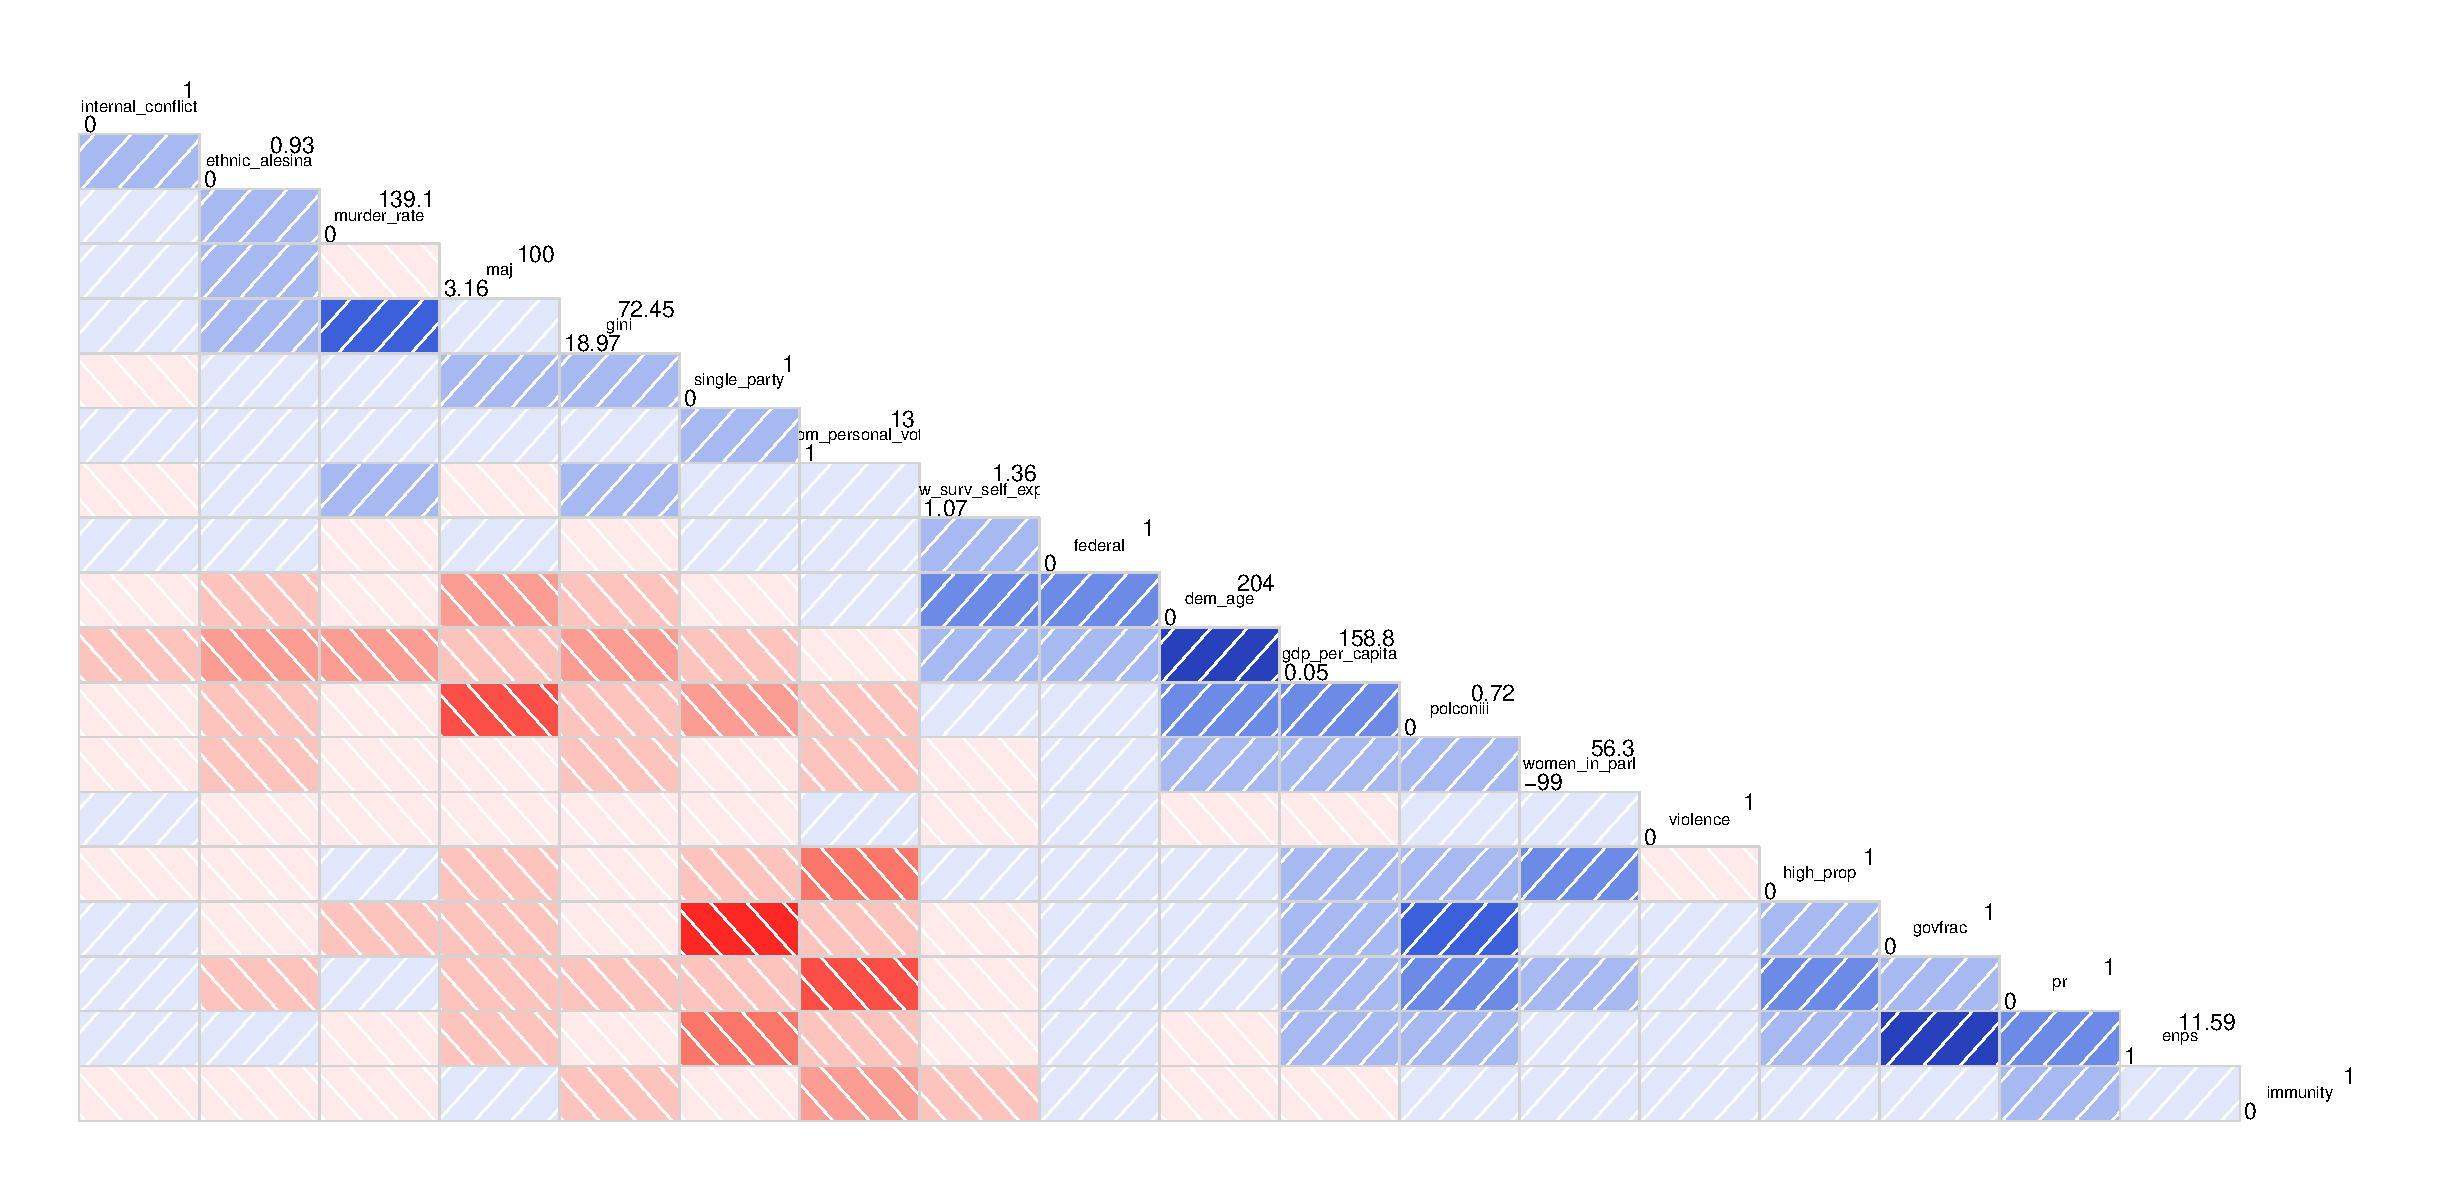
\includegraphics[scale=0.5]{corrScatter.pdf}

    \end{center}

    \caption{Correlation Matrix for Variables Included in the Analysis (Democratic Legislatures)}
    \label{corrmatrix}

    \begin{singlespace}
        {\scriptsize{Redder squares indicate stronger negative bi-variate correlations. \\
        Bluer squares indicate stronger positive bi-variate correlations. \\
        Numbers in the diagonal squares indicate the minimum and maximum observed values of the variables in the sample.
        }}
    \end{singlespace}
\end{figure}
\end{landscape}

%%%%%%%%%%%%%%%%%%%%%% Figures End %%%%%%%%%%%%%%%%%%%%%%%%%%%%%%%%%%%%%%%%%%%%%

\bibliographystyle{apsr}
\bibliography{LegViolence}

\end{document}
